\documentclass[mat1]{fmfdeloTS}

% do not add any definitions/commands before \zapisiMetaPodatke
% add appropriate text in the following commands 
\avtor{Carlo Lanzi Luciani} % Name Surname

\title{Groups of Automata and Grigorchuk Group} % English title
\naslov{Automatne Grupe in Grigorchuk Grup} % Slovenski naslov
\titolo{Gruppi di Automi e Gruppo di Grigorchuk} % Titolo italiano 

% names of advisors with full academic title: doc.~dr.~Ime Priimek,
% izr.~prof.~dr.~Ime Priimek, prof.~dr.~Ime Priimek
% use the correct command
\mentorja{izr. prof. dr. Ganna Kudryavtseva}{prof. Alessandro Logar}
% \mentorici{}{}

\letnica{2020} % year of degree


%  English abstract. Give a short description of the topic and results. 
\abstract{In this Final Thesis the reader will first get the basic notion of Word Space, Synchronous Automaton and their link with Tree Automorphism and the Wreath Product. After this short introduction we will see some examples of Automata which generate very interesting groups.}

%  Slovenian abstract. A more detailed description of the topic and results, amounting to at least 10 % of the length of the thesis.
\povzetek{}

% Italian abstract. Translation of the slovenian abstract.
\sintesi{}

% list at least one math subject classification code --
% these are available on www.ams.org/mathscinet/msc/msc2010.html
\klasifikacija{	20E07, 20E22, 	20E08, 	68Q70, 68Q45, 20E07, 20M35}

% Keywords. List relevant keywords that appear in the text
\keywords{Automata, Finite Automata, Word Spaces, Moore Diagram, Wreath Product,Grigorchuk, Burnside Problem} % english 
\kljucnebesede{Automata,Koncna Automata} % slovenian
\parolechiave{Automi, Automi Finiti} % italian

\zapisiMetaPodatke  % poskrbi za metapodatke in veljaven PDF/A-1b standard

%%%%%%%%%%%%%%%%%%%%%%%%%%%%%%%%%%%%%%%%%%%%%%%%%%%%%%%%%%%%%%%%%%%%%%%%%%%%%%%%%%%%%%%%%%%%%
%%%%%%%%%%%%%%%%%%%%%%%%%%%%%%%%%%%%%%%%%%%%%%%%%%%%%%%%%%%%%%%%%%%%%%%%%%%%%%%%%%%%%%%%%%%%%
%%%%%%%%%%%%%%%%%%%%%%%%%%%%%%%%%%%%%%%%%%%%%%%%%%%%%%%%%%%%%%%%%%%%%%%%%%%%%%%%%%%%%%%%%%%%%
%%%%%%%%%%%%%%%%%%%%%%%%%%%%%%%%%%%%%%%%%%%%%%%%%%%%%%%%%%%%%%%%%%%%%%%%%%%%%%%%%%%%%%%%%%%%%
%%%%%%%%%%%%%%%%%%%%%%%%%%%%%%%%%%%%%%%%%%%%%%%%%%%%%%%%%%%%%%%%%%%%%%%%%%%%%%%%%%%%%%%%%%%%%

% You can add your commands starting from here.
% Activate any packages you may need


%%°°°°°°°°°°°°°°°°°°°°°°°°°°°°°°°°°°°°°°°°°°°°°°°°
%%°°°°°°°°°°°°°°°°°°°°PACKAGES°°°°°°°°°°°°°°°°°°°°
\bibliographystyle{numeric}
\usepackage[utf8]{inputenc}
\usepackage{amsfonts,url}
\usepackage{verbatim}
\usepackage{amsmath}
\usepackage{tikz}
\usetikzlibrary{automata, positioning, arrows}
\usepackage{amssymb}
%%°°°°°°°°°°°°°°°°°°°°PACKAGES°°°°°°°°°°°°°°°°°°°°
%%°°°°°°°°°°°°°°°°°°°°°°°°°°°°°°°°°°°°°°°°°°°°°°°°


% Use the following symbols for number sets
\newcommand{\R}{\mathbb R}
\newcommand{\N}{\mathbb N}
\newcommand{\Z}{\mathbb Z}
\newcommand{\C}{\mathbb C}
\newcommand{\Q}{\mathbb Q}

% Declar mathematical operators so LaTeX will know how to typeset them
% \DeclareMathOperator{\conv}{conv}

% Add your definitions ...
%  \newcommand{}{}


%%°°°°°°°°°°°°°°°°°°°°°°°°°°°°°°°°°°°°°°°°°°°°°°°°
%%°°°°°°°°°°°°°°°°°°°°COMMANDS°°°°°°°°°°°°°°°°°°°°
\newcommand{\abece}{\mathbf X}
\newcommand{\fslovar}{\mathbf{X^*}}
\newcommand{\infslovar}{\mathbf{X^\omega}}
\newcommand{\auto}{\mathcal{A}}
\newcommand{\QQ}{\mathcal{Q}}
%%°°°°°°°°°°°°°°°°°°°°COMMANDS°°°°°°°°°°°°°°°°°°°°
%%°°°°°°°°°°°°°°°°°°°°°°°°°°°°°°°°°°°°°°°°°°°°°°°°


%%°°°°°°°°°°°°°°°°°°°°°°°°°°°°°°°°°°°°°°°°°°°°°°°°°°°°°
%%°°°°°°°°°°°°°°°°°°°°MATHOPERATORS°°°°°°°°°°°°°°°°°°°°
\DeclareMathOperator{\prefix{}}{\mathcal{P}}
\DeclareMathOperator{\aut}{\mathcal{AUT}}
\DeclareMathOperator{\Tran}{\mathcal{T}}
%%°°°°°°°°°°°°°°°°°°°°MATHOPERATORS°°°°°°°°°°°°°°°°°°°°
%%°°°°°°°°°°°°°°°°°°°°°°°°°°°°°°°°°°°°°°°°°°°°°°°°°°°°°

%---------------------------------------------------------------------------------------------------

\begin{document}

%---------------------------------------------------------------------------------------------------

% here starts the text of the Thesis
%%%%%%%%%%%%%%%%%%%%%%%%%%%%%%%%%%%%%%%%%%%%%%%%%%%%%%%%%%%%%%%%%%%%%%%%%%%%%%%%%%%%%%%%%%%%%
%%%%%%%%%%%%%%%%%%%%%%%%%%%%%%%%%%%%%%%%%%%%%%%%%%%%%%%%%%%%%%%%%%%%%%%%%%%%%%%%%%%%%%%%%%%%%
%%%%%%%%%%%%%%%%%%%%%%%%%%%%%%%%%%%%%%%%%%%%%%%%%%%%%%%%%%%%%%%%%%%%%%%%%%%%%%%%%%%%%%%%%%%%%
%%%%%%%%%%%%%%%%%%%%%%%%%%%%%%%%%%%%%%%%%%%%%%%%%%%%%%%%%%%%%%%%%%%%%%%%%%%%%%%%%%%%%%%%%%%%%
%%%%%%%%%%%%%%%%%%%%%%%%%%%%%%%%%%%%%%%%%%%%%%%%%%%%%%%%%%%%%%%%%%%%%%%%%%%%%%%%%%%%%%%%%%%%%


%%°°°°°°°°°°°°°°°°°°°°°°°°°°°°°°°°°°°°°°°°°°°°°°°°°°°°°
%%°°°°°°°°°°°°°°°°°°°°°°°°°°°°°°°°°°°°°°°°°°°°°°°°°°°°°
\tableofcontents
\section{Introduction}
Here we will cover the basic definitions necessary to comprehend the results and the examples.


%Add here graphics about how the topics are related between each other, following the example of APOSTOL, vol 2, beginning of the book


First we will see the concept of Word Space and his tree representation, then we will introduce the Semidirect Product, the Wreath Product  and some of its main characteristics. We will describe Asynchronous Automata, Synchronous ones, and finally the notion of group generated by an invertible, synchronous automaton.

%%°°°°°°°°°°°°°°°°°°°°°°°°°°°°°°°°°°°°°°°°°°°°°°°°°°°°°
\subsection{Word Spaces, Alphabet Trees and their Morphisms}
Let $\abece$ be a finite set with cardinality greater than 1, called the \textit{Alphabet}. From this derivate the mathematical concept of word:

\begin{definition}
$\fslovar:=\{x_1\dots x_n|n\in\N, x_i\in\abece \}$ is called the \textit{Set of Finite Words}.  The element with no letter is called the \textit{empty word}, and is written as $\varnothing$.


Given a word $w=x_1\dots x_n$, its lenght is $n$ and is written as $|w|=|x_1\dots x_n|$. The lenght of $\varnothing$ is 0.


$u \circ w=uw$ is the operation of \textit{concatenation}.
\end{definition}

\begin{proposition}
$(\fslovar, \circ)$ is a monoid, called the {Free Monoid}
\begin{proof}
The operation is obviously associative. $\varnothing$ represents the identity element of the semigroup, that is so a monoid.
\end{proof}
\end{proposition}

Later we will see that it is very useful to imagine this set in the form of a tree: the verteces are the elements of $\fslovar$ with $\varnothing$ as the root. We then say that $v$ is son of $u$ \texttt{if and only if} $u=vx$ for some $x\in \abece$. An example is \textbf{Fig. 1}.


\begin{figure}[ht]
\centering
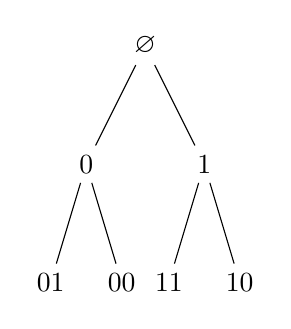
\begin{tikzpicture}

\node {$\varnothing$}
    child {  node {$0$}  child[right] { node {$01$} }
                    child[left] { node {$00$} } }
    child {  node {$1$}
                    child[right] { node {$11$} }
                    child[left] { node {$10$} }
             }  ;
\end{tikzpicture}
\caption{An example in the case $X=\{0,1\}$}
\label{Fig. 1}
\end{figure}

$X^n$, the set of the words of lenght $n$, is called the \textit{the n-th floor of $X^*$}(see \textbf{Fig.1})

Can a word with infinite letters exist? Can we reach the very bottom of the graph of \textbf{Fig. 1}?
\begin{definition}
The \textit{Set of Infinite Words} is $\infslovar:=\{x_1\dots x_i\dots|x_i\in \abece\}=\abece^{\N}$, also called the  \textit{Boundary tree}.
\end{definition}

\begin{proposition}
The concatenation can be extended, taking $u\in\fslovar$ and $v\in\infslovar$
\end{proposition}


Now we deal with some definition on words.
\begin{definition}
$w$ is the \textit{beginning \textit{, or} prefix} of a word $u\in\fslovar$(or $\infslovar$) if $u=wv$ for some $u\in\fslovar$(or $\infslovar$). In this case we set $v=u-w$

Given $A\in\fslovar\cup\infslovar$, we denote $\prefix{A}$ the longest common prefix of $A$, that is uniquely defined.

$v\in\infslovar$ is called \textit{almost periodic} if it is of the form $uwww\dots$
\end{definition}












In the future might be useful to have also some notion of topology on these spaces, in order to have some useful characterization of countinous function defined on them.

On $\infslovar$ we can introduce the product topology(taking on each $\abece$ the discrete topology), also known as the pointwise convergence topology. It's very easy to verify that the sets $w\infslovar:=\{wu|u\in\infslovar\}$ are clopen(closed and open) in this context.


We can also give a very useful characterization of distance. In fact for every decreasing sequence of positive numbers $\widetilde\lambda=(\lambda_n)_{n\in\N}$ such that $lim_{n\rightarrow\infty} \lambda_n =0$ we can find a metric $$d_{\widetilde\lambda}(w_1,w_2)=\lambda_n$$ defined on $\infslovar$, where $n=|\prefix{w_1,w_2}|$ is the longest common prefix of the words $w_1$ and $w_2$. This tell us that every $v\infslovar$ can be seen as a ball of radius $\lambda_{|w|}$ with the center on an arbitrary point $u\in v\infslovar$.



Finally we define the notion of homomorphism of trees, and some of their properties.

\begin{definition}
Given $A,B$ trees, $f: A\longrightarrow B$ is a \textit{tree homomorphism} if preserves the root and the adjacency of the tree, i. e.:
\begin{itemize}
\item If $a\in A$ is the root, $f(a)$ is the root
\item If $(u,v)$ is an edge of $A$, also $(f(u),f(v))$ is an edge of $B$
\end{itemize}
If $A=B$, $f$ is called \textit{endomorphism}.
If $A=B$ and $f$ is bijective we call it \textit{automorphism}.
\end{definition}
It's easy verifiable the the automorphism of a tree are a group.


\begin{proposition}
If $f$ is an endomorphism of tree $f(X^n)\subset X^n$
\end{proposition}
\begin{proof}
By induction on $n$
\end{proof}

We notice that every endomorphism $f:\fslovar(\infslovar)\longrightarrow\fslovar(\infslovar)$ can be uniquely extended to a continous map $f:\fslovar\cup\infslovar\longrightarrow\fslovar\cup\infslovar$. So each endomorphism in $\fslovar$ determines uniquely an endomorphism in $\infslovar$ and viceversa.

%%°°°°°°°°°°°°°°°°°°°°°°°°°°°°°°°°°°°°°°°°°°°°°°°°°°°°°
\bigskip
\bigskip
\bigskip
%%°°°°°°°°°°°°°°°°°°°°°°°°°°°°°°°°°°°°°°°°°°°°°°°°°°°°°
\subsection{Semidirect Products and Wreath Products}
These structures are complicated, but are extremely important to analyse the tipology of groups we are about to describe, so I advise to read this section carefully.
I would also like to underline, for the reader already familiar with these two concept, that we will use a notation inverted respect to western researchers, so:
\\Western Notation: $$A \wr B\quad A \rtimes_{\varphi}B$$
Here: $$B \wr A\quad B\ltimes_{\varphi}A$$
This choice is made because in the case of an infinite wreath or semidirect product is useful to have a finite number of symbols on our left.
Besides, every time we use the term \textit{action of a group} we assume \textit{action from the left}.



\begin{definition}
A \textit{permutational group} $(B,Y)$ is a group that can be embedded in $\mathcal{S} (Y)$, the permutation group of $X$.
\end{definition}

\begin{example}
\label{ex.1}
A typical example of permutational group is $(H,N)$ where $N\triangleleft H$ and the faithful action performed by $H$ is:
$$s:(h,n)\longmapsto hnh^{-1}$$
\end{example}


\begin{definition}
A \textit{faithful action} $f: G\times X\longrightarrow X$ is an action such that, given $g\neq h$ in $G$, exists $x\in X$ for which $gx\neq hx$.
\end{definition}
\begin{proposition}
$G$ acts faithfully on $X$ if and only if $(G,X)$ is a permutational group.
\end{proposition}
\begin{proof}
$(\Rightarrow)$: we can easily verify it through $\Phi:G\longrightarrow \mathcal{S}(X)$ defined by $\Phi(g)=\phi_g$ where $\phi_g(x):=gx$.
$(\Leftarrow)$ obvious
\end{proof}

So having a faithful action of $G$ on $X$ or a permutational group $(G,X)$ is exactly the same thing.


\begin{proposition}
In general if $X$ is a group $\aut(X)\subsetneq\mathcal{S}(X)$. So in general if $(G,X)$ is a permutational group and $X$ is a group, the injective endomorphism $G\longrightarrow\mathcal{S}(X)$ \textit{doesn't} induce an endomorphism $G\longrightarrow\aut(X)$.
\end{proposition}

\begin{example}
In the example \ref{ex.1} instead, $s$ induces an endomorphism $H\longrightarrow\aut(N)$ because for each $h$, the application $h\longmapsto hnh^{-1}$ is also an automorphism.
\end{example}


\begin{definition}
Given two groups $H,N$, with operations $\ast_H$ and $\ast_N$ and an homomorphism $\varphi:H\longrightarrow \aut(N)$, where $\aut(N)$ is the group $\{ f:N\longrightarrow N | f\quad is \quad bijective\}$, we can define on the set $H\times N$ the subsequent operation:
\[
\star_\varphi:((h_1,n_1),(h_2,n_2))\longmapsto (\quad h_1\ast_H h_2\quad,\quad n_1\ast_N(\varphi(h_1))(n_2)\quad)
\]
We call $(H\times N,\star_\varphi)$ the  \textit{Semidirect Product of $N,H$ relative to $\varphi$} and we write it down as $H\ltimes_{\varphi} N$.
\end{definition}

\begin{proposition}
$H\ltimes_{\varphi} N$ is a group, where the identity is $(1_H,1_N)$ and, for each $(h,n)$ the inverse is $(h^{-1},(\varphi(h))(n^{-1}))$.
\end{proposition}


\begin{example}
Always working on \ref{ex.1} we have a common example of Semidirect Product. We've been given $H,N$ groups and $\varphi:H\longrightarrow\aut(N)$ in which $\varphi(h)=\varphi_h$ where $\varphi_h(n)=hnh^{-1}$. The semidirect product $H\ltimes_\phi N$ is $(H\times N, \star_\varphi)$ has $(1_H,1_N)$ as identity and, for each $(h,n)$, the inverse $(h^{-1},(\varphi(h))(n^{-1}))\quad=\quad(h^{-1},hn^{-1}h^{-1})$
\end{example}


Now we did the first step. In oreder to the second we must work a little bit more.

\begin{definition}
Given a group $A$ and an arbitrary set of indexes $Y$ we define:
\begin{itemize}
\item 
\begin{description}
The \textit{Direct Product}
$A^Y = \prod_{\omega\in Y} A:=\{ \overline{a}=(a_\omega )_{\omega\in Y} : a\in A\}$
\end{description}
\item 
\begin{description}
The \textit{Direct Sum} 
$A^{(Y)} = \bigoplus_{\omega\in Y} A:=\{ \widetilde{a}=(a_\omega )_{\omega\in Y} : a\in A \wedge a\neq 1_A$ just for a finite number of indexes $\}$
\end{description}
\end{itemize}
We can naturally extend the operation of $A$ on the two structures component-wise, to obtain so another 'bigger' group.
\end{definition}


Now let's take $(A,X),B$ groups, where $(A,X)$ is a permutational group. If we construct $A^{Y}$ we have a group on which $B$ can act faithfully, so we have an injective homomorphism $\Phi : B\longrightarrow \mathcal{S}(A^Y)$, through the action of $B$ on the indexes of $A^Y$. \\
If we prove that $\Phi(B)\subset\aut(A^Y)$ we have everything we need to construct $B\ltimes_{\Phi} A^{Y}=H\ltimes_{\varphi} N$. The same con be done substituting $A^{Y}$ with $A^{(Y)}$.
\\
Let's formalise this:

\begin{proposition}
Given $(B,Y)$ and $A$ groups, with $(B,Y)$ permutation group, we can extend the action of $B$ on $A^Y$, so $(B,A^Y)$ is a permutational group. Plus, $B$ is a subgroup of $\aut(A^Y)$.\\
The same con be done substituting $A^{Y}$ with $A^{(Y)}$.
\end{proposition}
\begin{proof}
If $by$ is the action of $B$ on $Y$, we can define the action of $B$ on $A^Y$ as follow:
$$q(b,\overline{a})=q_b(\overline{a})=b\overline{a}=b(a_y)_{y\in Y}:=(a_{by})_{y\in Y}$$
\begin{enumerate}
\item We have to prove that $q$ is a faithful, i.e. that $q_b\in\mathcal{S}(A^Y)$:
if $\overline{a}=(a_y)_{y\in Y}\neq(x_y)_{y\in Y}=\overline{x} \Rightarrow \exists y'\in Y$ such that $a_{y'}\neq x_{y'}$. Let's now look $q_b(\overline{a})$ at the index $by'$. We find $a_{by'}$, different from $x_{by'}$, that is the $by'$-th component of $q_b(\overline{b})$. So $q_b$ is injective. The surjectivity is very simple: if we have $(a_y)_{y\in Y}$ the element $(a_{b^{-1}y})_{y\in Y}$ is its counter-image.
\item We have now to prove that $q_b$ is an automorphism: $q_b(\overline{a}\star\overline{x})=q_b((a_y\star x_y)_{y\in Y})=(a_{by}\star x_{by})_{y\in Y}=(a_{by})_{y\in Y}\star (x_{by})_{y\in Y}=q_b(\overline{a})\star q_b(\overline{x})$
\end{enumerate}
\end{proof}

\begin{definition}
Given a permutational group $(B,Y)$ and a group $A$ we can define two structure of Wreath Product as follows:
\begin{itemize}
\item The \textbf{\underline{Unrestricted}} or \textbf{\underline{Complete}} \textbf{Wreath Product}, so the semidirect product on $(B,A^{Y})$ where the required homomorphism is an application $\varphi:B\longrightarrow \mathcal{S}(A^Y)$ defined by $(\varphi(b))(\overline{a}=(a_y)_{y\in Y})=(a_{by})_{y\in Y}$
\item The \textbf{\underline{Restricted}} \textbf{Wreath Product}, so the semidirect product on $(B,A^{(Y)})$ where the required homomorphism is an application $\varphi:B\longrightarrow \mathcal{S}(A^{(Y)})$ defined by $(\varphi(b))(\widetilde a=(a_y)_{y\in Y})=(a_{by})_{y\in Y} $
\end{itemize}
We write them both as $B\wr A$, the distiction will be understandable from the context.
\end{definition}
\textbf{Note:} If we take a two group $B,A$ we can anyway consider their wreath product considering $(B,B)$ a permutational group, where $B$ acts faithfully on himself by left multiplication.



\begin{example}
\textit{The Lamplighter Group.} This famous example is the restricted wreath product $\Z\wr\Z_2$. The \textit{base} of the wreath product is $(\Z,\bigoplus_{j\in\Z} ({\Z_2})_j)$, and the operation is:
$$(z_1, (a_{j})_{j\in\Z})\star(z_2, (b_{j})_{j\in\Z}):=(z_1+z_2, (a_j+_{\Z_2}b_{z_1+j})_{j\in\Z})$$
\end{example}
%%°°°°°°°°°°°°°°°°°°°°°°°°°°°°°°°°°°°°°°°°°°°°°°°°°°°°°
\bigskip
\bigskip
\bigskip
%%°°°°°°°°°°°°°°°°°°°°°°°°°°°°°°°°°°°°°°°°°°°°°°°°°°°°°
\subsection{Asynchronus Automata}
%%°°°°°°°°°°°°°°°°°°°°°°°°°°°°°°°°°°°°°°°°°°°°°°°°°°°°°
The word comes from greek \textit{automaton}(plural \textit{automata \textit{or} automatons}), and means "acting on one's self-will". For this reason the plural can also be \textit{automata}, over the english-logical automatons.
The idea of an Automaton is "machine" in which we plug an input and we receive an output. They are what computer scientist call a "mathematical model for computation". The formal definition is:

\begin{definition}
An \textbf{Asynchronous  Automaton} is a set $\auto=<X_I,X_O,\QQ,\pi,\lambda>$ where:
\begin{itemize}
	\item $X_I$ and $ X_O $ are \textit{finite} sets called respectively the \textit{\textbf{Input \emph{and} Output Alphabets}}
	% so here we declare what we put inside and what comes aoutside of the machine
	\item $\QQ$ is a set called the \textit{\textbf{Set of Internal States of the  Automaton}}
	\item $\pi:X_I\times\QQ \longrightarrow \QQ $ is a function called the \textit{\textbf{Transition Function}}
	\item $\lambda:X_I\times\QQ \longrightarrow X_O $ is a function called the \textit{\textbf{Output Function}}
\end{itemize}
If $\QQ$ is finite we call $\auto$ a \textit{finite automaton} or a \textit{finite state automaton}. If $|\lambda(x,q)|=1\quad \forall x,q$ we call the Automaton \textbf{synchronous}.
\end{definition}

So our automaton is a structure of a machine that, for each state, and for each input, travel through a sequence of states and spit an output. How do we imagine this idea? Well, we can \textit{see} it:

\begin{definition}
Given an Automaton $\auto=<X_I,X_O,\QQ,\pi,\lambda>$ we define his \textbf{Moore Diagram} as the oriented graph $G=(\QQ, \mathcal{E})$ where the set of the edges $(q_1,q_2)$ are connected whenever $\exists x\in X_I\quad s.t.\quad\pi(x,q_1)=q_2$ and the label reffered to each edge is $x|\lambda(x,q_1)$(=input|output). 
\end{definition}

We observe that for every automaton his Moore Diagram has this characteristic:
\begin{equation}
\forall q\in\QQ\textrm{ and }\forall x\in X_{I} \quad\exists! e\in\mathcal{E} \textrm{ such that the left side of its label reads "}x\textrm{"}\label{(1)}
\end{equation}

I thank Edward F. Moore, for he gave us an easy-manageable representation of these objects.
We can see here an example, in order to appreciate Mr. Moore:
\begin{figure}[ht]
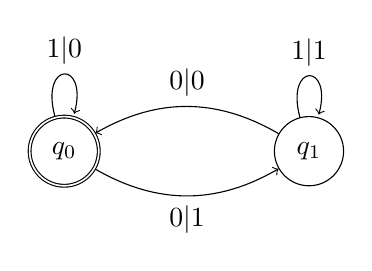
\begin{tikzpicture}
\node[state, accepting](q0) at (0,0) {$q_0$};
\node[state, right of=q0, xshift=60] (q1) {$q_1$};
\draw	(q0) edge[below,bend right,->] node{$0|1$} (q1)
		(q0) edge[loop above] node{$1|0$} (q0)
		(q1) edge[loop above] node{$1|1$} (q1)
		(q1) edge[above, bend right,->] node{$0|0$} (q0);
		
\end{tikzpicture}
\caption{Example of a Moore Diagram of a 2-state Synchonous Automaton over the alphabet $X_I=X_O=X=\{0,1\}$}
\label{Fig. 2}
\end{figure}


%conjecture to verify
These Diagram are so fantastic also because whenever a graph respects the condition \ref{(1)}, it uniquely defines an automaton. So if $S$ is the set of these graphs, there is a unique correspondence between $S$ and the set of all Automaton. This means that, in case of Finite Automata, instead of defining this types of machine through some tedious list of outputs for each possible inputs, we can simply draw them. To compute the outcome of the transition function or the output one, given an input and a state, we just follow the arrows and we make the product of the the left sides of the labels.

\begin{proposition}
We can naturally extend the Domain of $\pi$ and $\lambda$:
\begin{itemize}
	\item $\pi:X_{I}^{*} \times \QQ:\longrightarrow \QQ $
	$$\pi(\varnothing,q)=q$$ $$\pi(w x,q)=\pi(w,\pi(x,q))$$
	\item $\lambda:X_{I}^{*} \times \QQ:\longrightarrow X_{O}^{*}$
	$$\lambda(\varnothing,q)=\varnothing$$ $$\lambda(w x,q)=\lambda(w,\pi(x,q))\lambda(x,q)$$
\end{itemize}
\end{proposition}
So now, for every state $q$, we're able to plug in entire words(entities in $\fslovar$ and not necessarily just in $\abece$) and obtain words. What if we fix $q$?

\begin{definition}
If an  Automaton $\auto$ has a fixed state $q_0$ we call it an \textit{Initial  Automaton} and we write it as $\auto_{q_0}$. Each $\auto_{q_0}$ naturally defines $f:{X_I}^*\longrightarrow {X_O}^*$, with $f(w):=\lambda(w,q_0)$, called \emph{Action of the  Automaton $\auto_{q_0}$}.
\end{definition}

\begin{definition}
Two Initial Automata are said to be \textit{equivalent} if they define the same actions.
\end{definition}


If an Automaton is the skeleton, an Initial Automaton is an alive working machine, that for each input gets an output travelling through the states. In fact an Automaton doesn't define any function, till we don't fix a state $q_0$.

Now let's select just the type of machines interesting to us.
\begin{definition}
An Initial Automaton $\auto_{q_0}$ is \textit{accessible} if $\forall q\in\QQ$ exists a word $w\in X_I$ such that $\pi(w,q_0)=q$.
\end{definition}
From now on we will deal just with \textit{accessible} automata.

%MAYBE i WILL PUT THE VARIOUS RESULT OF THE ACTION OF THE NONDEGENERATE AUTOMATON AND SO ON, WITH ALL THE DEFINITION OF THE MODIFIED AUTOMATON.

%I WOULD ANYWAY SKIP ALL THE PART ON REDUCED AND MINIMAL AUTOMATA, BUT I WOULD LIKE TO DEAL WITH CONTINOUS FUNCTION AND SPACES X\OMEGA
We want to start working with something algebraic. We'll do that in a few steps.
\begin{definition}
Given $\auto_1=<X_I,X_{IO},\QQ_1,\pi_1,\lambda_1>$ and $\auto_2=<X_{IO},X_O,\QQ_2,\pi_2,\lambda_2> $ we define their \emph{composition} $\mathcal{B}=\auto_1*\auto_2=<X_I,X_O,\QQ_1\times\QQ_2,\pi,\lambda>$ with $\pi$ and $\lambda$ as follows:
\begin{itemize}
\item $\pi(x,(s_1,s_2))=(\pi_1(x,s_1),\pi_2(\lambda_1(x,s_1),s_2))$
\item $\lambda(x,(s_1,s_2))=\lambda_2(\lambda_1(x,s_1),s_2)$
\end{itemize}
\textbf{Observe:}
(Action of $\auto_2$)$\circ$(Action of $\auto_1$)=Action of $\auto_1*\auto_2$
\end{definition}
This is something similar to put two machine in serie. Informally means we feed the second machine with the output of the first one, as the observation suggests. We notice also that:

\begin{proposition}
The actions of the Initial Automata in which $X_I=X_O$ form a semigroup.
\end{proposition}
%%°°°°°°°°°°°°°°°°°°°°°°°°°°°°°°°°°°°°°°°°°°°°°°°°°°°°°
\bigskip
\bigskip
\bigskip
%%°°°°°°°°°°°°°°°°°°°°°°°°°°°°°°°°°°°°°°°°°°°°°°°°°°°°°
\subsection{Mealy Automata}

Mealy automata is simply a synonimous of Synchronous Automaton, so an automaton such that $|\lambda(x,q)|=1$ for every $x,q$. 

A few notes:
\begin{itemize}
\item From now on we will consider just automata such that $X=X_I=X_O$.
\item in the Moore diagram of the Synchronous Automata notation is often more "spontaneous", and often arrows are subscribed with just the left side of the label.
\end{itemize}

\begin{definition}
A \textit{Moore Automaton} is a Mealy Automaton in which exists $\mu:\QQ\longrightarrow X_O$ such that $\lambda(x,q)=\mu(\pi(x,q))$
\end{definition}
\begin{proposition}
For every Mealy automaton exists an equivalent Moore automaton
\end{proposition}

\begin{proposition}
The transformations on $\fslovar$ defined by the Mealy Automata form a semigroup $\mathcal{SF(X)}$. Besides, the semigroup of actions on $\infslovar$ by the same automata is to $\mathcal{SF(X)}$ isomorphic.
\end{proposition}
\begin{proof}
For the first point is sufficient to notice that a compostion of Mealy automata is a Mealy automaton. For the second point we see that, in the case of the Mealy Automata an action on $\fslovar$ uniquely determines an action on $\infslovar$ and viceversa. So follow for their compositions.
\end{proof}

Let's focus on this semigroup $\mathcal{SF(X)}$. The contained transformations are called¸\textit{synchronous automatic}. We want to explore their properties.
\begin{definition}
A transformation $f:\fslovar\longrightarrow\fslovar$ is said to \textit{preserve common beginnings of words} if $\forall u,w\in\fslovar$ is valid$$|\mathcal{P}\{u,w\}|\leq|\mathcal{P}\{f(u),f(w)\}|$$
\end{definition}
\begin{proposition}
$f$ is synchronous automatic \textit{if and only if} preserves lenght of words and common beginnings.
\end{proposition}



%%°°°°°°°°°°°°°°°°°°°°°°°°°°°°°°°°°°°°°°°°°°°°°°°°°°°°°
\bigskip
\bigskip
\bigskip
%%°°°°°°°°°°°°°°°°°°°°°°°°°°°°°°°°°°°°°°°°°°°°°°°°°°°°°
\subsection{Groups of Automata}
%%°°°°°°°°°°°°°°°°°°°°°°°°°°°°°°°°°°°°°°°°°°°°°°°°°°°°°








%%°°°°°°°°°°°°°°°°°°°°°°°°°°°°°°°°°°°°°°°°°°°°°°°°°°°°°
%%°°°°°°°°°°°°°°°°°°°°°°°°°°°°°°°°°°°°°°°°°°°°°°°°°°°°°
%%°°°°°°°°°°°°°°°°°°°°°°°°°°°°°°°°°°°°°°°°°°°°°°°°°°°°°




\cite[p.~8-32]{Grigor}
\bigskip
\bigskip
\bigskip
\bigskip
\begin{thebibliography}{99}

\bibitem{Nekrash}
Volodymyr Nekrashevych, \textbf{Self-similar groups}, International University Bremen, School of Engineering and Sci-
ence, P.O. Box 750 561, 28725 Bremen, Germany

\bibitem{Grigor}
R. I. Grigorchuk, V. V. Nekrashevich, V. I. Sushchanskii \textbf{Automata, Dynamical Systems and Groups}, Proceedings of the Steklov Institute of Mathematics, Vol. 231, 2000, pp. 128-203
%\bibitem{}

\bibitem{WreathEncMat}
Wreath product, \textit{Encyclopedia of Mathematics} URL: http://www.encyclopediaofmath.org/

\end{thebibliography}

\end{document}

